\documentclass[12pt]{article}

\usepackage{/Users/ryanbaker/cxxsaturdays/tex/preamble}

\begin{document}

\begin{center}

\Huge\textbf{Pointers}

\vspace{1em}

\LARGE\textbf{Introduction to Modern C++}

\vspace{1em}

\Large{Ryan Baker}

\vfill

\includegraphics[width=0.5\textwidth]{\rootdir/tex/images/logo.png}

\end{center}

\vfill

\tableofcontents

\pagebreak

\section{Pointers}

\noindent
One of the major appeals of C++ is the ability to work with memory directly.
At the heart of this feature lies the concept of pointers.
A \textbf{pointer} is a variable that holds a memory address--often the address of another variable.
Pointers ``point to'' locations in memory and allow indirect access and manipulation of the data stored there.

\subsection{Declaring and Defining Pointers}

\noindent
Pointers are declared in relation to the type of data they point to.
This is important: the compiler needs to know what type of value a pointer refers to so it knows how many bytes to read and how to interpret them.
To declare a pointer, use an asterisk \inlinecxx{*} along with the type:

\begin{cxx}{}
int*    p1; // declares a pointer to an int
char*   p2; // declares a pointer to a char
double* p3; // declares a pointer to a double
\end{cxx}

\noindent
A brief aside: there's frequent debate over whether to write \inlinecxx{int* ptr} or \inlinecxx{int *ptr} when declaring pointers.
Both forms are valid and functionally identical--the choice comes down to coding style and personal preference.

\begin{advice}
\noindent
I tend to prefer \inlinecxx{int* ptr} because, conceptually, I think of \inlinecxx{int*} as its own data type: ``pointer to \inlinecxx{int}''.
However, this style can introduce a subtle pitfall when declaring multiple variables on the same line:

\begin{cxx}{}
int* p1, p2;  // p1 is a pointer, p2 is an int
int *p1, *p2; // p1 is a pointer, p2 is a pointer
int* p1, *p2; // p1 is a pointer, p2 is a pointer
\end{cxx}

\noindent
Because of this ambiguity, many developers advocate for the second style--\inlinecxx{int *ptr}--as a more honest representation of how the C++ parser actually reads the declaration.
Personally, I find this case fringe enough to dismiss.
I tend to believe we should prioritize how humans read the declaration over how the parser does.

\end{advice}

\subsubsection{Address-Of Operator \inlinecxx{&}}

\noindent
To define a pointer that ``points to'' a variable, we use the \textbf{address-of operator} \inlinecxx{&} to fetch the address of that variable:

\begin{cxx}{}
int x;
int* ptr { &x }; // ptr points to x
\end{cxx}

\noindent
When we write \inlinecxx{&x}, we're asking C++ to give us the memory address where \inlinecxx{x} lives.
This address is just a number--somewhat like a street address--that tells us where we can find the value of \inlinecxx{x} in memory.
Addresses are typically shown in hexadecimal:

\begin{cxx}{addressof.cpp}
#include <iostream>

int main()
{
	int x;
	std::cout << &x << std::endl;
}
\end{cxx}

\begin{terminal}
$ clang++ -std=c++23 addressof.cpp && ./a.out
0x16db9ed7c
\end{terminal}

\subsubsection{Dereference Operator \inlinecxx{*}}

\noindent
To access the value pointed to by a pointer, we prefix the pointer with the \textbf{dereference operator} \inlinecxx{*}:

\begin{cxx}{}
int* ptr;
int x { *ptr }; // assigns x to the value pointed to
\end{cxx}

\noindent
Here's a more complete example of pointer dereferencing in action:

\begin{cxx}{dereference.cpp}
#include <iostream>

int main()
{
	int x { 42 };
	int* ptr { &x };
	std::cout << "x = " << *ptr << std::endl;
}
\end{cxx}

\begin{terminal}
$ clang++ -std=c++23 dereference.cpp
$ ./a.out
x = 42
\end{terminal}

\noindent
When we write \inlinecxx{*ptr} we're telling C++: ``go to the address stored in \inlinecxx{ptr}, and give me the value that resides there."
Since pointers provide direct memory access, they can also be used to modify variables indirectly:

\begin{cxx}{increment.cpp}
#include <iostream>

int main()
{
	int x { 42 };
	int* ptr { &x };
	(*ptr)++;
	std::cout << "x = " << x << std::endl;
}
\end{cxx}

\begin{terminal}
$ clang++ -std=c++23 increment.cpp && ./a.out
x = 43
\end{terminal}

\subsection{\inlinecxx{NULL} Pointers}

\noindent
A \textbf{null pointer} is a pointer that does not point to any valid memory address, typically represented by memory address 0.
In C, \inlinecxx{NULL} is a preprocessor macro that resolves to \inlinecxx{0}.
In C++, the \inlinecxx{nullptr} keyword was introduced to provide a type-safe representation of a null pointer, replacing \inlinecxx{NULL}.
Therefore, all of the following are valid ways to define null pointers:

\begin{cxx}{}
int* p { 0 };
int* q { NULL };
int* r { nullptr };
\end{cxx}

\noindent
In C++-land, \inlinecxx{int* r \{ nullptr \};} is typically preferred for better type safety and clarity.

\vspace{1em}
\noindent
We use \inlinecxx{NULL} pointers because a pointer that points to nothing is safer than one that points to anything.
As we'll soon see, stack memory is not default-initialized, meaning the following code:

\begin{cxx}{}
int main() {
	int* ptr;
}
\end{cxx}

\noindent
creates a pointer that points to a (virtually) random address.
Dereferencing this pointer before it's been initialized can cause a program-ending memory error--or worse, it might appear to work just fine, leading to a subtle runtime bug because you've accidentally manipulated memory you didn't intend to touch.

\begin{advice}
\noindent
For this reason, it's always a good idea to initialize pointers at the time of declaration.
If there's no meaningful address to give them, use \inlinecxx{nullptr}.

\begin{cxx}{}
int* ptr { nullptr };
\end{cxx}

\noindent
This gives your program more deterministic behavior and allows it to fail fast and cheaply, reducing the chances of subtle bugs.
\end{advice}

\subsubsection{Dereferencing Null Pointers}

\noindent
Since a null pointer doesn't point to a valid memory address by definition, attempting to read or write through it results in undefined behavior.
In most cases, this will manifest as a segmentation fault:

\begin{cxx}{nullptr.cpp}
#include <iostream>

int main()
{
    int* ptr { nullptr };
    std::cout << *ptr << std::endl;
}
\end{cxx}

\begin{terminal}
$ clang++ -std=c++23 nullptr.cpp
$ ./a.out
[1]    23783 segmentation fault  ./a.out
\end{terminal}

\noindent
For this reason, if safety is critical and there's a chance a pointer might be null, you should always provide appropriate handling by checking for null before deferencing:

\begin{cxx}{}
if (ptr != nullptr && *ptr /* ... */)
\end{cxx}

\noindent
Some functions and algorithms return \inlinecxx{nullptr} to indicate failure or the absence of a result.
So, checking for null before dereferencing is essential to avoid undefined behavior.

\vspace{1em}
\noindent
One interesting note: null pointer dereferencing is allowed within the \inlinecxx{sizeof} operator because the operand isn't actually evaluated:

\begin{cxx}{}
int* ptr { nullptr };
std::cout << sizeof(*ptr) << std::endl; // legal!
\end{cxx}

\subsection{Pointer Arithmetic}

Pointers support various arithmetic operations that allow for navigation through memory.
These operations fall into two broad categories: operations between pointers and integers, and operations between pointers themselves.

\begin{itemize}

	\item \textbf{Pointer + Integer}: Addition and subtraction (which includes increment and decrement).
	\item \textbf{Pointer - Pointer}: Pointer subtraction and comparison.

\end{itemize}

\noindent
Pointers can be incremented or decremented.
Importantly, arithmetic on a \inlinecxx{T*} respects the size of \inlinecxx{T}.
So, moving a pointer by an integer value adjusts its address by \inlinecxx{sizeof(T)} bytes, not just one byte.
For example, if \inlinecxx{sizeof(int)} = 4, then incrementing an \inlinecxx{int*} will move it by four bytes:

\begin{center}
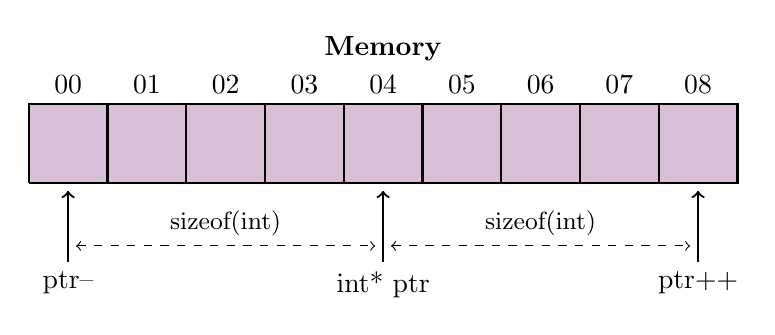
\begin{tikzpicture}
	\fill[Thistle] (0,0) -- ++(9,0) -- ++(0,1) -- ++(-9,0) -- ++(0,-1);
	\draw[thick]
	(0,0) -- ++(0,1) -- ++(9,0) -- ++(0,-1) -- ++(-9,0)
	(1,0) -- ++(0,1)
	(2,0) -- ++(0,1)
	(3,0) -- ++(0,1)
	(4,0) -- ++(0,1)
	(5,0) -- ++(0,1)
	(6,0) -- ++(0,1)
	(7,0) -- ++(0,1)
	(8,0) -- ++(0,1)
	(0.5,1) node[above] { 00 }
	(1.5,1) node[above] { 01 }
	(2.5,1) node[above] { 02 }
	(3.5,1) node[above] { 03 }
	(4.5,1) node[above] { 04 }
	(5.5,1) node[above] { 05 }
	(6.5,1) node[above] { 06 }
	(7.5,1) node[above] { 07 }
	(8.5,1) node[above] { 08 }
	(4.5,1.7) node {\textbf{Memory}}
	;
	\draw[->,thick] (4.5,-1) -- ++(0,0.9);
	\draw[->,thick] (0.5,-1) -- ++(0,0.9);
	\draw[->,thick] (8.5,-1) -- ++(0,0.9);
	\draw (4.5,-1) node[below] {\inlinecxx{int* ptr}};
	\draw (0.5,-1) node[below] {\inlinecxx{ptr--}};
	\draw (8.5,-1) node[below] {\inlinecxx{ptr++}};
	\draw[<->,dashed] (0.6,-0.8) -- ++(3.8,0);
	\draw[<->,dashed] (4.6,-0.8) -- ++(3.8,0);
	\draw (2.5,-0.8) node[above] {\small\inlinecxx{sizeof(int)}};
	\draw (6.5,-0.8) node[above] {\small\inlinecxx{sizeof(int)}};
\end{tikzpicture}
\end{center}

\begin{cxx}{ppp.cpp}
#include <iostream>

int main()
{
	int* p { nullptr };
	std::cout << p++ << ',' << p++ << ',' << p << '\n';
}
\end{cxx}

\begin{terminal}
$ clang++ -std=c++23 ppp.cpp
$ ./a.out
0x0,0x4,0x8
\end{terminal}

\noindent
Similarly, adding an integer $n$ to a pointer will adjust the pointer by \(n \times \texttt{\textcolor{Cerulean}{sizeof}(T)}\) bytes.
You can think of this as moving the pointer by $n$ elements, where each element is of type \inlinecxx{T}, assuming elements of that type are stored contiguously in memory.

\begin{cxx}{padd.cpp}
#include <iostream>

int main()
{
	short* p { nullptr }; // sizeof(short) == 2

	std::cout << p << ',';
	p += 4;
	std::cout << p << ',';
	p -= 3;
	std::cout << p << std::endl;
}
\end{cxx}

\begin{terminal}
$ clang++ -std=c++23 padd.cpp
$ ./a.out
0x0,0x8,0x2
\end{terminal}

\begin{explanation}
\noindent
When we add 4 to \inlinecxx{p}, \inlinecxx{p} is advanced by $4 \times \texttt{\textcolor{Cerulean}{sizeof}(\textcolor{BurntOrange}{short})} = 8$ bytes, or 4 elements.
Similarly, when we subtract 3 from \inlinecxx{p}, it is advanced by $-3 \times \texttt{\textcolor{Cerulean}{sizeof}(\textcolor{BurntOrange}{short})} = -6$ bytes, or $-3$ elements.
\end{explanation}

\noindent
Subtracting two pointers of the same type will yield the number of elements between them--not the number of bytes.
Given two pointers \inlinecxx{T* p1}, \inlinecxx{T* p2}, and letting $B$ representing the difference in bytes between them, we get:

\[\texttt{p1} - \texttt{p2} = \frac{B}{\texttt{\textcolor{Cerulean}{sizeof}(T)}}\]

\noindent
In cases where the pointers are not properly aligned--that is, their addresses are not even multiples of \inlinecxx{sizeof(T)}--the division truncates toward 0:

\begin{cxx}{misaligned.cpp}
#include <iostream>

int main()
{
    int* p1 { (int*)1002 };
    int* p2 { (int*)1000 };
    std::cout << (p1 - p2) << std::endl; // 0
}
\end{cxx}

\noindent
Here's a more realistic example demonstrating how pointer subtraction can be used to determine the number of elements between two variables:

\begin{cxx}{psub.cpp}
#include <iostream>

int main()
{
	int a, b, c, d, e, f;
	int* p1 { &a };
	int* p2 { &f };

	std::cout << (p1 - p2) << std::endl;
}
\end{cxx}

\begin{terminal}
$ clang++ -std=c++23 psub.cpp
$ ./a.out
5
\end{terminal}

\begin{note}
The exact value may vary depending on how variables are laid out on the stack, but this example assumes contiguous allocation in declaration order (which is common, though not guaranteed).
\end{note}

\vspace{0.99em}
\noindent
Pointers of the same type can be compared using standard relational operators like \inlinecxx{==}, \inlinecxx{!=}, \inlinecxx{<}, \inlinecxx{>}, \inlinecxx{<=}, and \inlinecxx{>=}.
The result of such comparisons depends solely on the memory addresses the pointers hold:

\begin{cxx}{pcomp.cpp}
#include <iostream>

int main()
{
	int* p1 { nullptr }; 
	int* p2 { p1 + 1 };

	if (p1 < p2)
		std::cout << "p1 points to a lower address\n";
	else if (p1 == p2)
		std::cout << "p1 and p2 point to the same address\n";
	else
		std::cout << "p1 points to a higher address\n";
}
\end{cxx}

\begin{terminal}
$ clang++ -std=c++23 pcomp.cpp
$ ./a.out
p1 points to a lower address
\end{terminal}

\subsection{Pointers to Pointers}

\end{document}
